\documentclass[PMO,authoryear,lsstdraft,toc]{lsstdoc}
% lsstdoc documentation: https://lsst-texmf.lsst.io/lsstdoc.html
% \input{meta}

% Package imports go here.

% Local commands go here.

%If you want glossaries
%\input{aglossary.tex}
%\makeglossaries

\title{Summit Computing Cluster}

% Optional subtitle
% \setDocSubtitle{A subtitle}

\author{%
Cristian Silva
}

\setDocRef{ITTN-061}
\setDocUpstreamLocation{\url{https://github.com/lsst-it/ittn-061}}

\date {\today}

% Optional: name of the document's curator
% \setDocCurator{The Curator of this Document}

\setDocAbstract{%
Description of the deployment of the summit computing cluster. 
}

% Change history defined here.
% Order: oldest first.
% Fields: VERSION, DATE, DESCRIPTION, OWNER NAME.
% See LPM-51 for version number policy.
\setDocChangeRecord{%
  \addtohist{1}{YYYY-MM-DD}{Unreleased.}{Cristian Silva}
}


\begin{document}

% Create the title page.
\maketitle
% Frequently for a technote we do not want a title page  uncomment this to remove the title page and changelog.
% use \mkshorttitle to remove the extra pages

% ADD CONTENT HERE
% You can also use the \input command to include several content files.
\section{Introduction}


The original concept for the \CC was to put it at the base in La Serena (\cite[Sec. 9]{LDM-148}),
but there are a number of problems with this:
\begin{itemize}
\item
  Data taken on the summit would have to be transferred to the base, and ingested into a separate butler
\item
  We would have to install, and maintain, a batch processing system at the base (including managing
  the butler registry)
\item
  Some of the functionality provided by the \CC is needed to monitor the survey data quality,
  and it is not clear that the summit-base link is reliable enough to guarantee that the results of this
  analysis will always be available at the summit.  Depending on the definition of `degraded mode' this
  may or may not be a problem
\end{itemize}

Accordingly, we propose that the \CC nodes be moved to the summit, to augment a pre-existing cluster, yagan.
We note that much of the most compute-intensive work during commissioning is expected to be carried out at
USDF (\cite{RTN-021}).
The benefits of this modified topology for the IT group include:
\begin{itemize}
    \item Reduced administration overhead 
    \item Limit security constraints to a single location
    \item Simplifies configuration deployment
    \item Promotes summit independence 
\end{itemize}
The big picture of the current topology is the following:

\begin{figure}
    \centering
    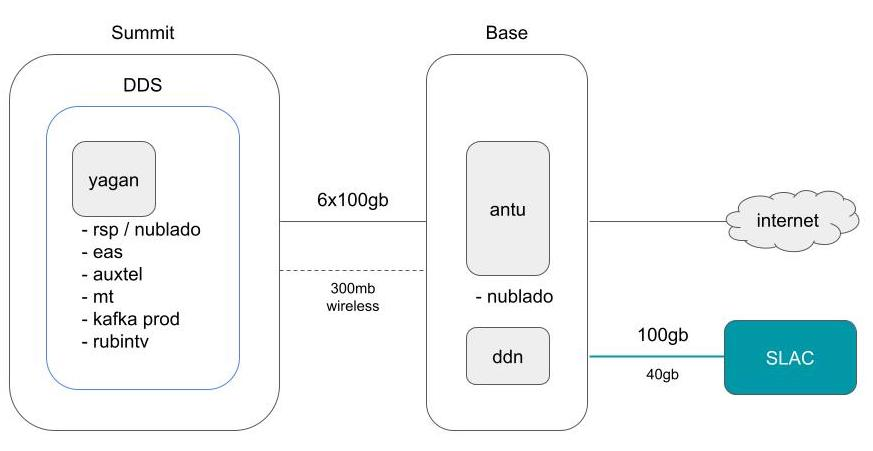
\includegraphics[width=18cm]{images/current_state.jpg}
    \caption{topology}
\end{figure}

\newpage

\section{Current State}

\subsection{Hardware}

The commissioning cluster runs in the antu nodes, with a capacity of 832 cores and 3.2TB of Ram. Details of its hardware configuration can be found in \href{https://ittn-014.lsst.io/}{ITTN-014 Computing Infrastructure}

\begin{figure}
    \centering
    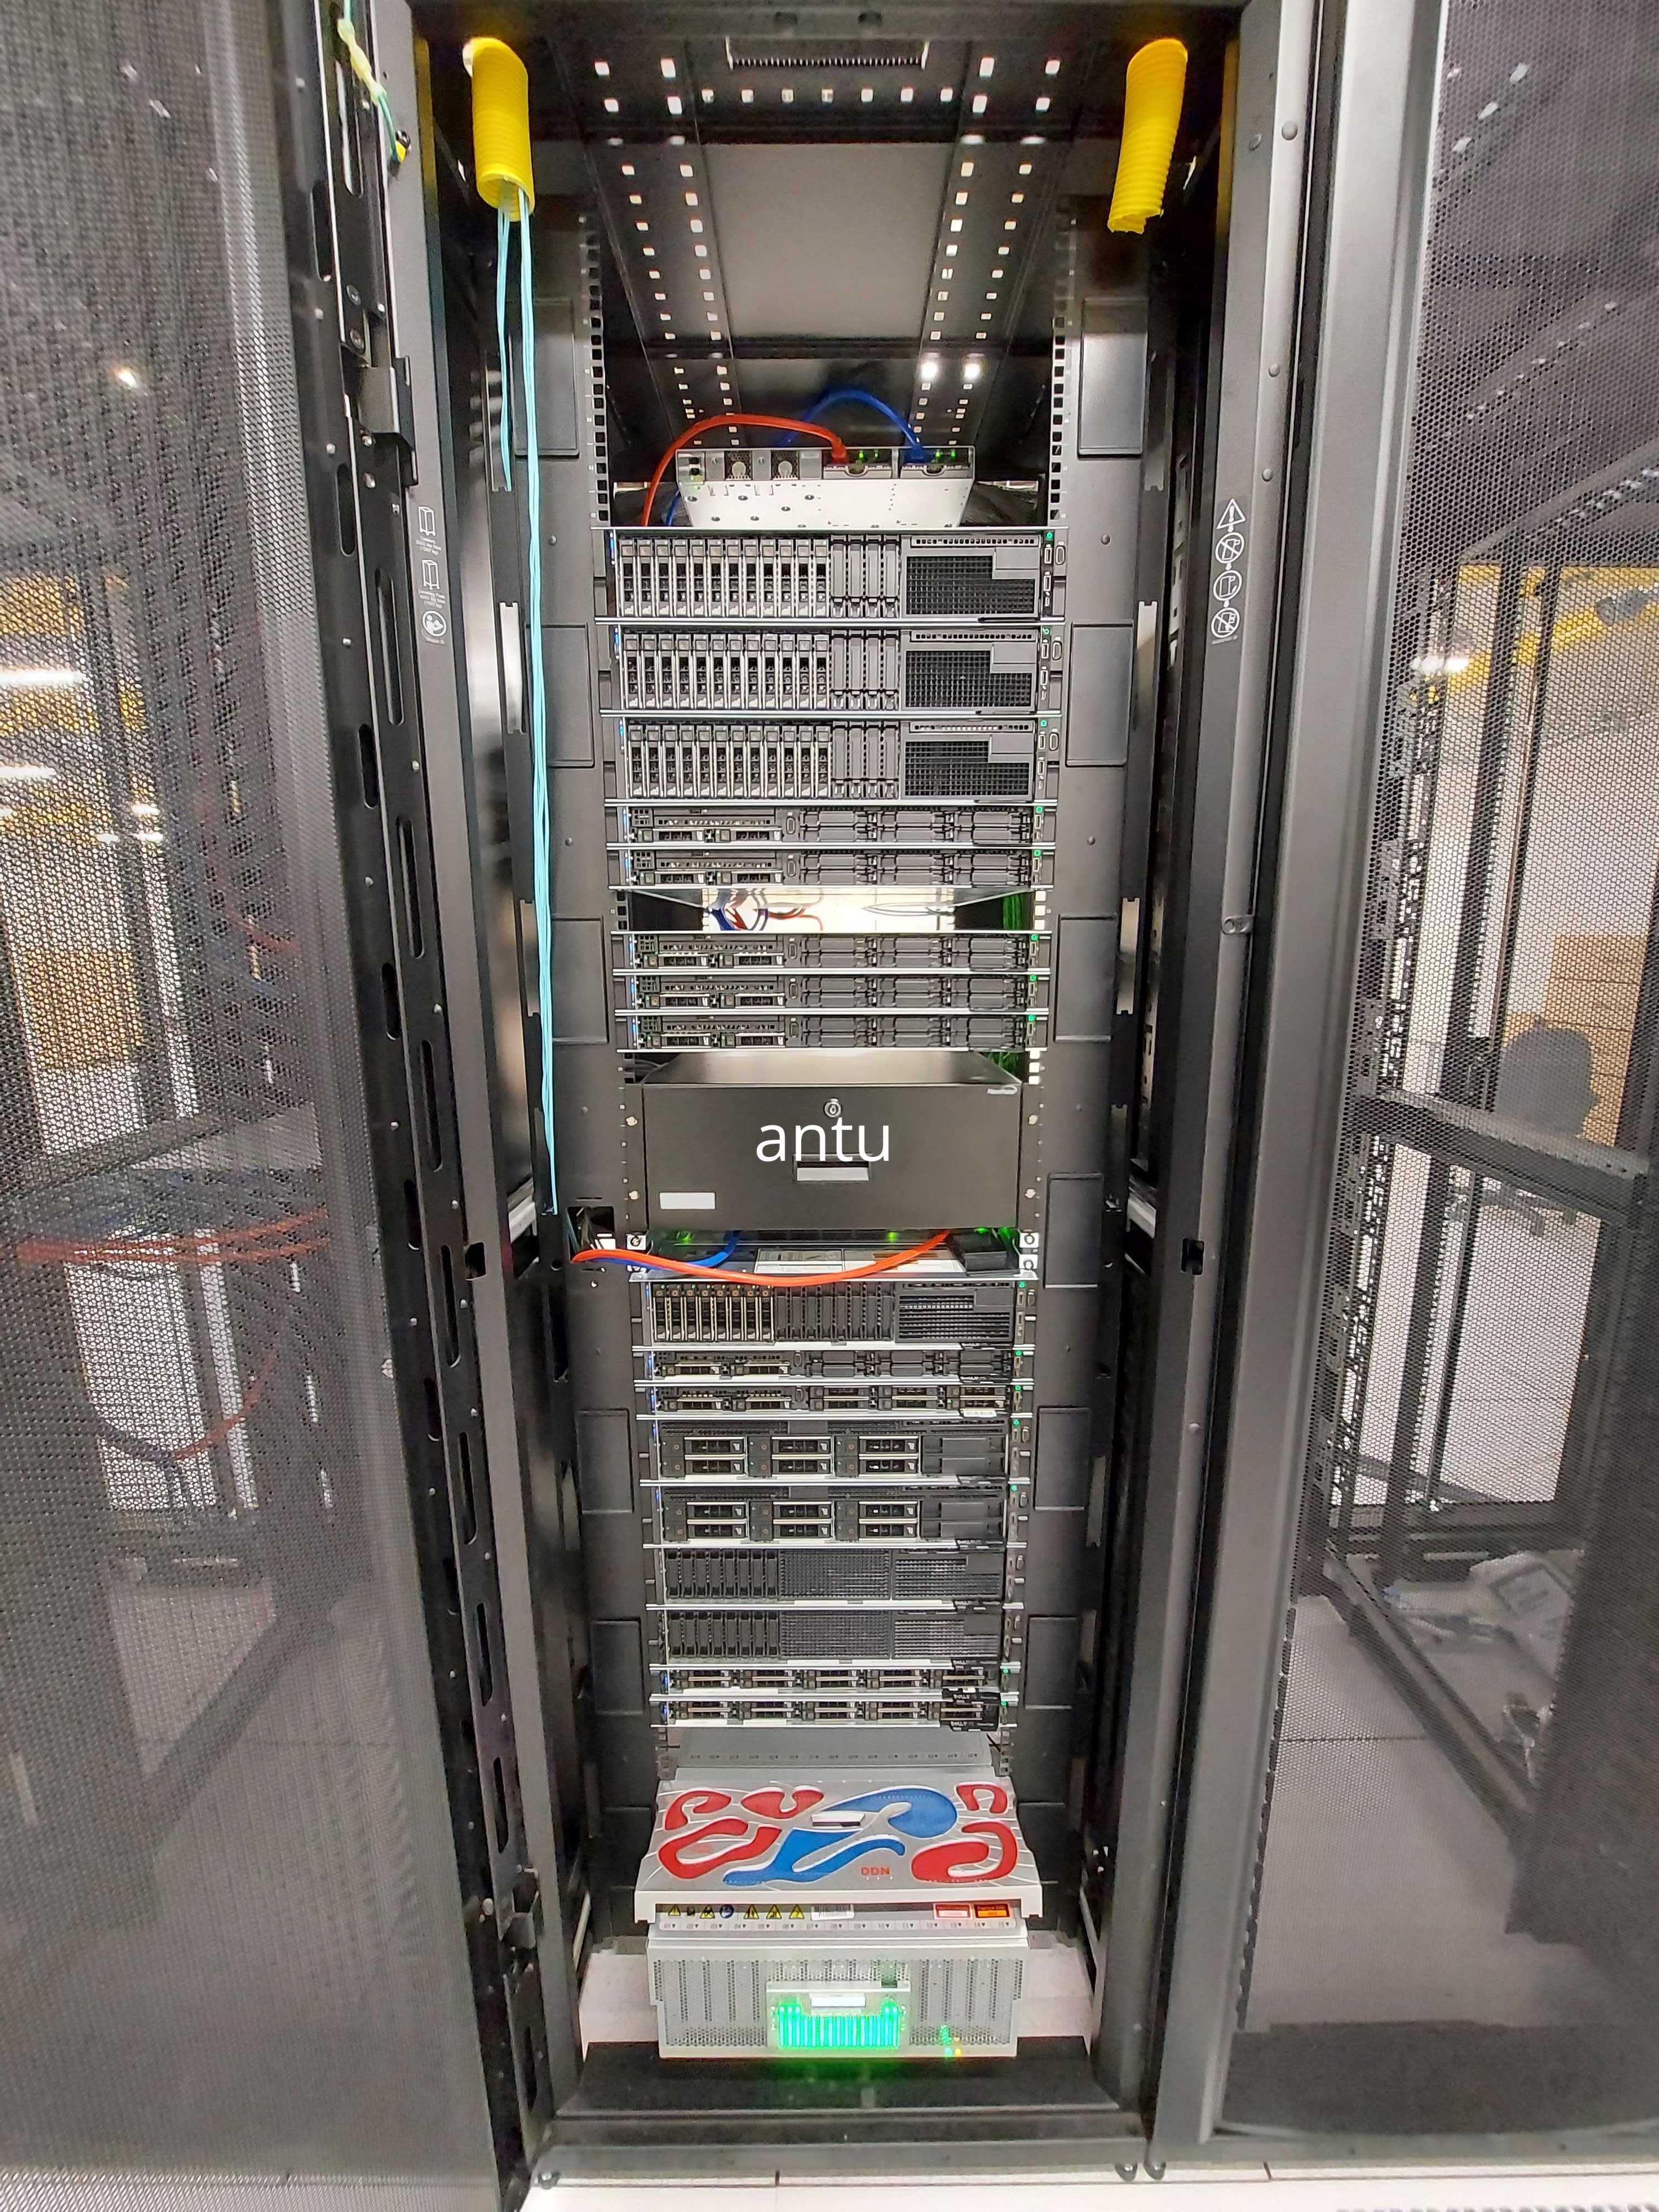
\includegraphics[width=10cm]{images/antu.jpg}
    \caption{antu cluster}
\end{figure}

The servers composing the antu cluster are a mix of different Dell models, previously deployed as forwarders and DTNs by NCSA. There's also a DDN unit of about 700TB of storage, and it is currently providing NFS mounts for Nublado
\newpage

The computing cluster at the summit is called yagan. It has a capacity of 576 cores and 2.2TB of Ram. 

\begin{figure}
    \centering
    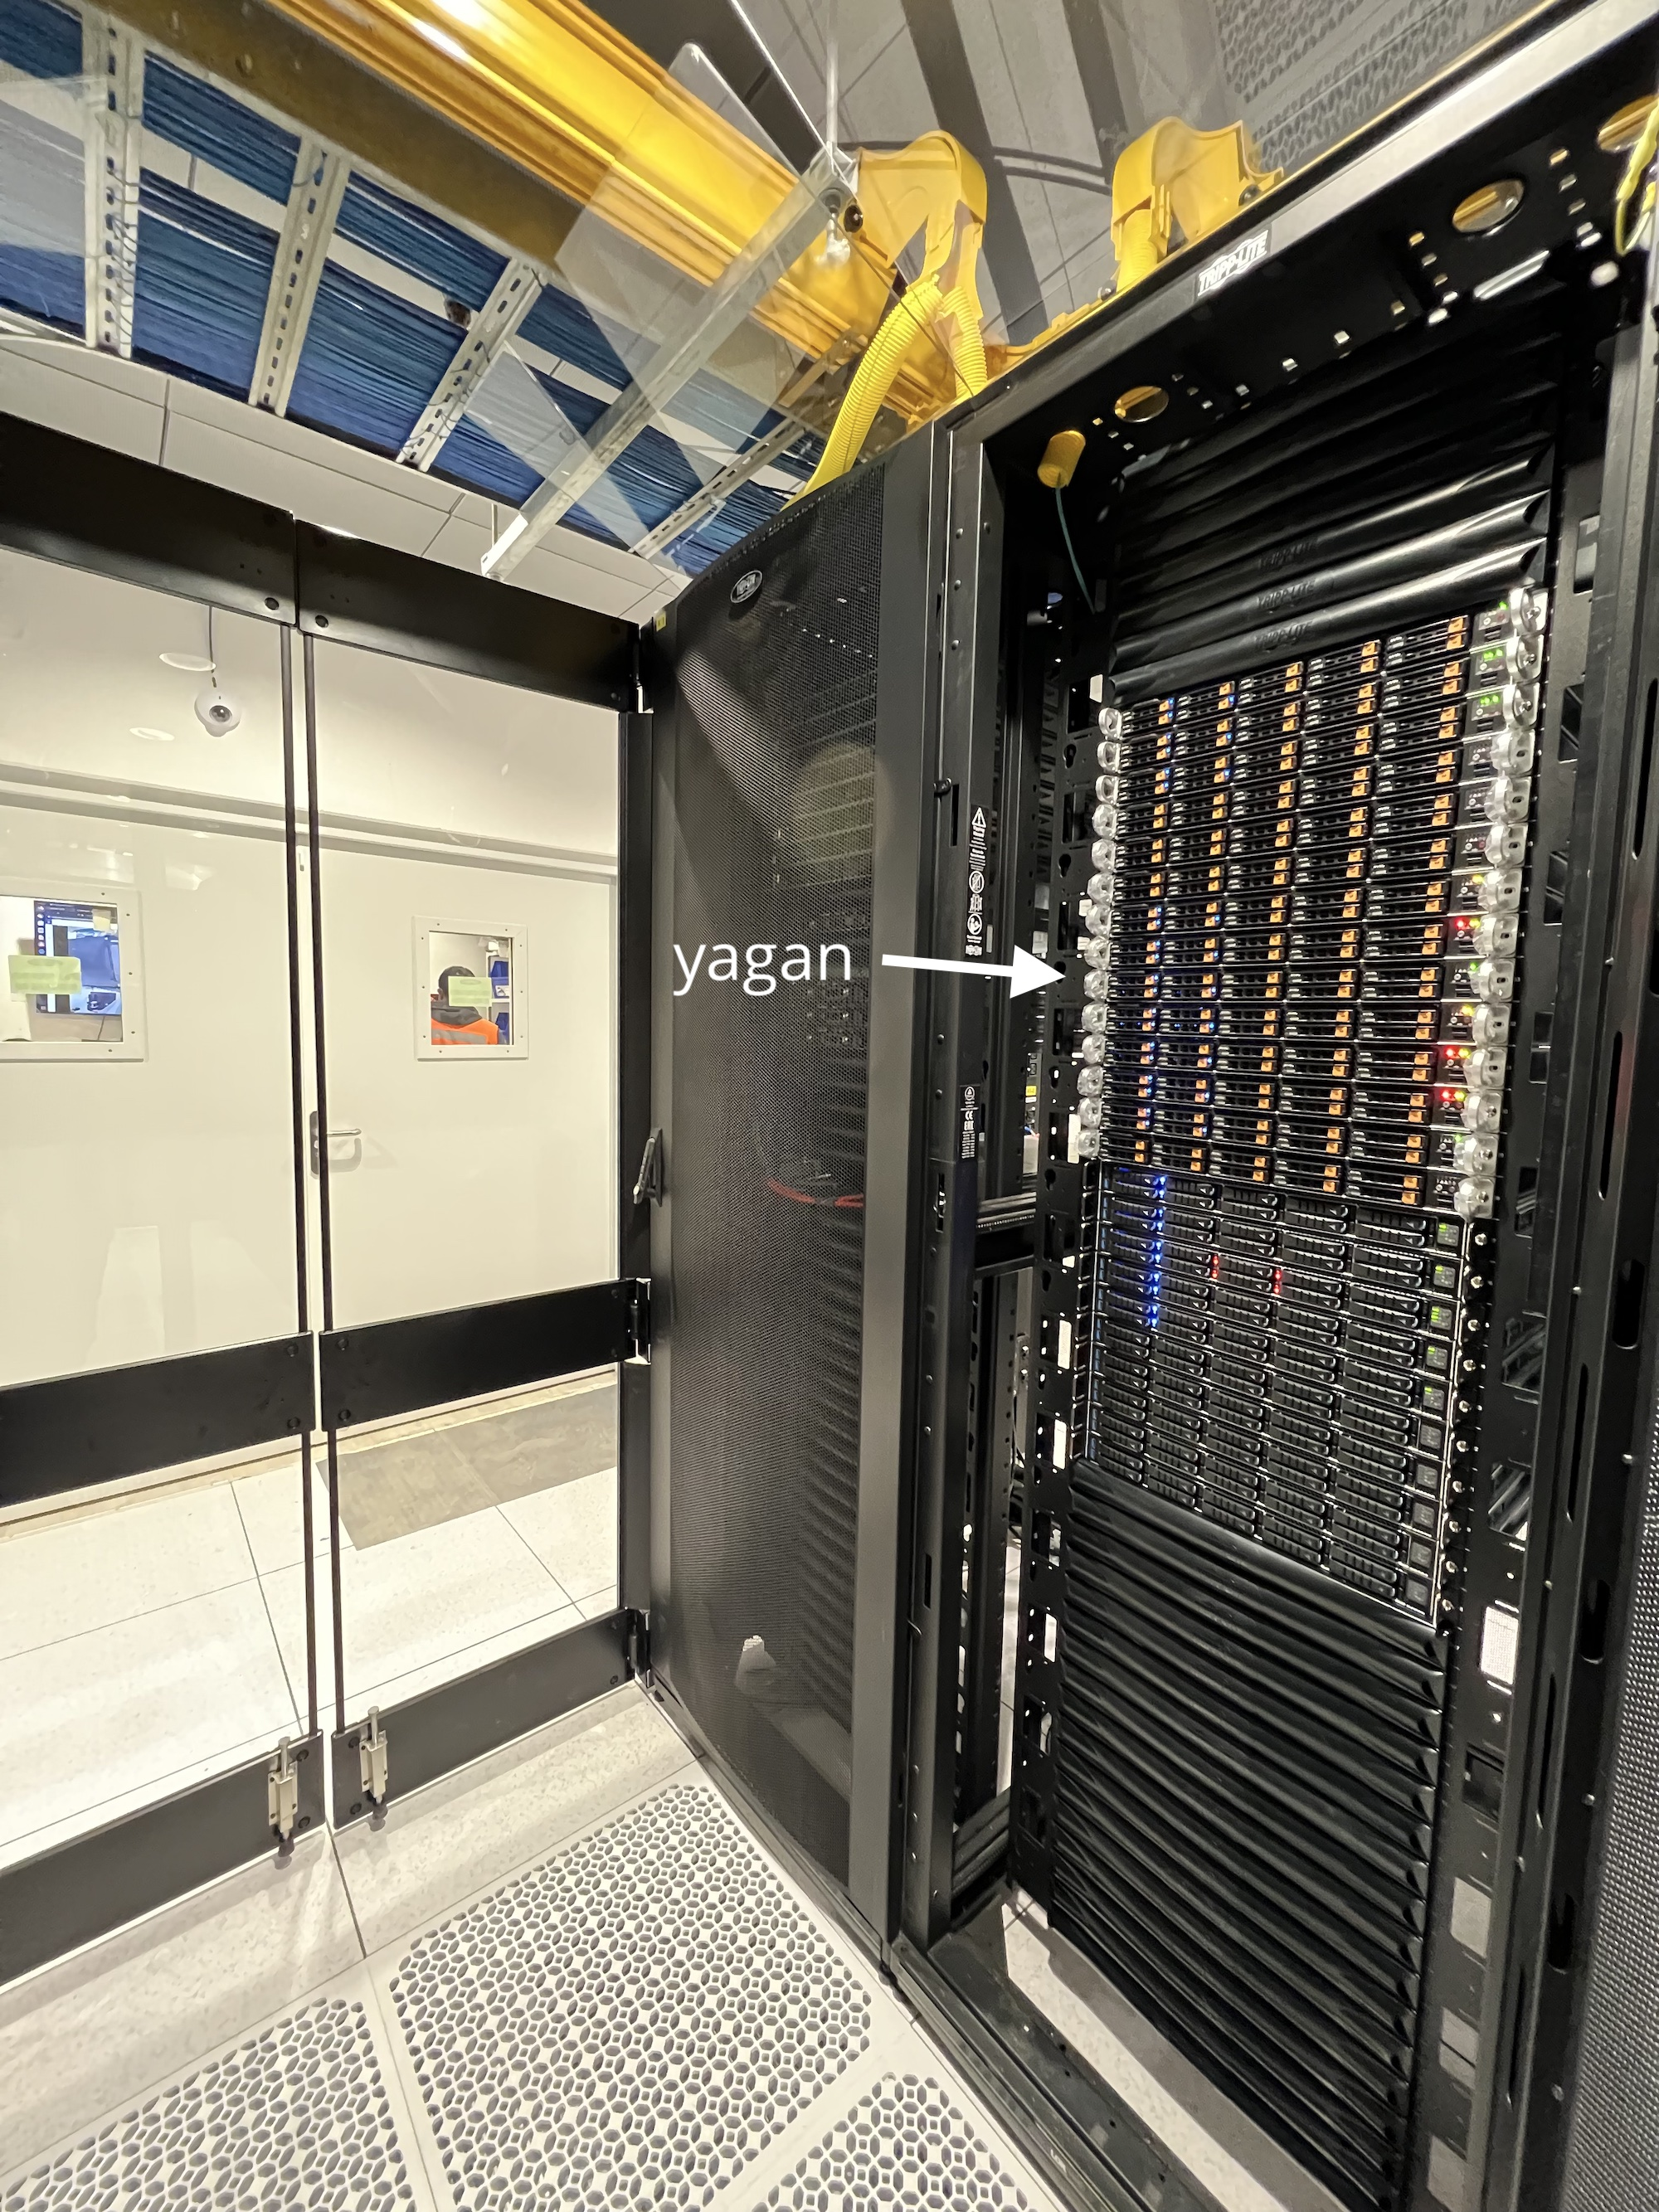
\includegraphics[width=10cm]{images/yagan.jpg}
    \caption{clusters at the summit}
\end{figure}

The servers in the yagan cluster have the same model and specs. This hardware model is shared with several other services and clusters at the summit, so they all work as a big pool of spares in case a node fails.  

\newpage

\subsection{Software}

All clusters are provisioned using  Rubin Devops Stack (puppet, ipa, etc)

The antu cluster runs:
\begin{itemize}
    \item Nublado
\end{itemize}

The yagan cluster runs: 
\begin{itemize}
    \item Rubin Science Platform
    \item EFD (in migration process)
    \item EAS CSCs
    \item Auxtel CSCs
    \item Kafka Producers 
    \item MT CSCs
    \item RubinTV
\end{itemize}

Regardless of the several components running in yagan, its cpu usage stays below 10\% and the RAM usage is never above 5\%


\section{Planned State}

Each rack at the summit has a maximum of 48RU, 8RU are used by network equipment such as switches and fiber headers. Therefore each rack could potentially host 40 servers of 1RU each.

The kubernetes clusters at the summit are all of 1RU with 64 cores; hence each rack could deliver up to 2500 cores. However, given the current commissioning and summit cluster size, the maximum size of the new computing cluster would be 1400 cores. 



\appendix
% Include all the relevant bib files.
% https://lsst-texmf.lsst.io/lsstdoc.html#bibliographies
\section{References} \label{sec:bib}
\renewcommand{\refname}{} % Suppress default Bibliography section
\bibliography{local,lsst,lsst-dm,refs_ads,refs,books}

% Make sure lsst-texmf/bin/generateAcronyms.py is in your path
\section{Acronyms} \label{sec:acronyms}
\addtocounter{table}{-1}
\begin{longtable}{p{0.145\textwidth}p{0.8\textwidth}}\hline
\textbf{Acronym} & \textbf{Description}  \\\hline

CC & Change Control \\\hline
DDN & Data Delivery Network \\\hline
EAS & Environmental Awareness System \\\hline
EFD & Engineering and Facility Database \\\hline
IT & Information Technology \\\hline
LDM & LSST Data Management (Document Handle) \\\hline
MT & Main Telescope \\\hline
NCSA & National Center for Supercomputing Applications \\\hline
NFS & Network File System \\\hline
OODS & Observatory Operations Data Service \\\hline
PMO & Project Management Office \\\hline
PanDA &  Production ANd Distributed Analysis system \\\hline
RAM & Random Access Memory \\\hline
RTN & Rubin Technical Note \\\hline
USDF & United States Data Facility \\\hline
\end{longtable}

% If you want glossary uncomment below -- comment out the two lines above
%\printglossaries





\end{document}
